\chapter{Literature Review}\label{chapter:lit}

This chapter introduces to traditional and Deep Learning approaches of image synthesis, and overviews ways of inferring DNNs in real-time on mobile devices. Sections \ref{lit:traditional-cg} and \ref{lit:nrender} gradually expand on state-of-the-art reconstruction of human images, with more attention to the parts that comprise the basis for this work. The used metrics and optimization losses are described in Section \ref{lit:metrics}. Then, methods for decreasing DNNs inference time are given (Section \ref{lit:dnn-speedup}) with a few peculiarities of the mobile devices targeted by this work (Section \ref{lit:mobile}).

\section{Traditional 3D representations and rendering algorithms}
\label{lit:traditional-cg}

Ever since the dawn of Computer Graphics, many primitive representations for 3D world were proposed to reconstruct real objects. The representations may model volumetric properties, such as occupancy, density of matter, radiance, color at a certain point of 3D space; or model surfaces and assign these properties to points on a surface. The definition of the primitives may be explicit or implicit. An explicit surface can be defined by taking every point on a real coordinate plane $\mathbb{R}^2$, and mapping it to the third "height" coordinate explicitly via function $f_e(.) \in \mathbb{R}$. An implicit surface is defined by a zero-level set of a multivariable function $f_i(.) \in \mathbb{R}$ \cite{survey:advances-nn22}.
\begin{multicols}{2}
\setlength\abovedisplayskip{0pt}
\noindent
\begin{equation}
	\renewcommand\arraystretch{0.6}
	S_{explicit} = \left\{ 
	\left( \begin{array}{c} x \\ y \\ f_{e}(x,y) \end{array} \right) \Bigg\rvert 
	\left( \begin{array}{c} x \\ y \end{array} \right) \in \mathbb{R}^2
	\right\}
\end{equation}
\begin{equation}
	\renewcommand\arraystretch{0.6}
	S_{implicit} = \left\{ \begin{pmatrix} x \\ y \\ z \end{pmatrix} \in \mathbb{R}^3 \Bigg\rvert f_{i}(x, y, z) = 0 \right\}
\end{equation}
\setlength\belowdisplayskip{0pt} 
\end{multicols} 

Unlike surfaces, values of volumetric properties are usually defined only explicitly for all points in the 3D space:

\begin{equation}
	\renewcommand\arraystretch{0.6}
	V = \left\{ f_{vol}(x,y,z)  \Bigg\rvert \begin{pmatrix} x \\ y \\ z \end{pmatrix} \in \mathbb{R}^3 \right\}
\end{equation}
  

Let's look at the common surface and volume representations in details. A \textit{point cloud} is a discrete set of points in $\mathbb{R}^n$ (usually $\mathbb{R}^3$). It can model either surfaces (thus each point belongs to the surface) or volumes. The points may be associated with additional attributes, such as: color, density, orientation vector (normal) of a surface. When rendering an image from a point cloud, commonly the points are interpreted as spheres with a certain radius, in order to compensate for sparsity and lack of connectivity between adjacent points \cite{aux:pointcloud21}.

A \textit{polygonal mesh} is the most wide-spread 3D representation, being a compromise between granularity of 3D modeling and computational requirements to render adequate images. It reconstructs curvature of a surface using small planar segments, usually triangles or quads, and generally $N$-sided polygons. A set of 3D points (vertices) is defined, along with enumeration of connected vertices. Although each vertex can be associated with additional attributes, using \textit{textures} much finer details can be modeled. Usually, textures are 2D images, that store in the pixels values of attributes (color, surface orientation, etc). Each 3D vertex on a mesh has designated 2D texture coordinates (also referred to as UV-coordinates; See Figure \ref{intro:fig:mesh-texture}). A barycentric interpolation of vertices' texture coordinates is used to sample an attribute value from the texture for a certain point on a polygon. Textures allow to model details, that are too hard to approximate directly with polygons, e.g. small wrinkles, folds of clothes, complex color patterns, etc. Using textures, a variety of information can be modeled, e.g. a normal direction to an abstract fine-detailed surface for all points on polygons, allowing to calculate realistically looking interaction of light with materials, without additional computational overhead \cite{aux:normal-mapping78}. 

A \textit{voxel grid} is commonly referred to as a 3D image, for also being a regular grid of primitives - cubes (voxels) with associated attributes. As volumetric representations, they may store occupation or density of matter at all points in a closed 3D area \cite{aux:voxels98}. Voxel grids are fast to process, but are enormously large in memory. Storing fine-detailed geometry requires shrinking the grid's scale, but memory consumption grows cubically. Thus, attempts on sparse voxel grids were made, using hyerarchical structures, that are longer to query, but can encapsulate large empty space into very large voxels, and reconstruct fine details using very small voxels where needed \cite{aux:voxels-sparse13}.

\textit{Implicit functions}, as already described, can model surfaces. For example, we can define a Signed Distance Function for all points in a 3D volume. The values tell the closest distance to the surface, with negative sign if the point is "inside" a surface. However, to render an image, the surface (i.e. the zero-distance set) has to be queried repeatedly from the implicit representation. This makes image synthesis computationally expensive, unless an intermediate explicit representation is built to approximate the surface, e.g. using Marching Cubes algorithm \cite{aux:marching-cubes87} to reconstruct a mesh.

The computer graphics evolution led to computing hardware to support some 3D representations. For instance, images are now typically rendered using Graphic Processing Units (GPUs), that unlike general Central Processing Units (CPUs) implement operations of linear algebra in a massively parallel way, allowing to process millions of primitives in real-time. Next, we'll describe the most common rendering algorithms called \textit{ray casting} and \textit{rasterization}. They can be adapted to any 3D representation, although sometimes with too high computational complexity.

For both algorithms, a virtual camera is mathematically modeled. In physical cameras, light that bounces in the 3D space forms an image as it hits the camera's sensor. Light can be captured from a larger span of view using lenses, that focus light rays into a single spot, referred to as camera origin or focal point. For virtual cameras, a pinhole model is used, where a focal point is chosen, and the 3D scene representation is projected on a pixel grid, as if it was placed at a distance from the focal point, called focal length. From that, a view \textit{frustum} is defined, that is a pyramid that extends from the focal point through the image to infinity, and has apex cut off at the focal length. Objects outside the frustum are invisible to the virtual camera. See Figure \ref{lit:fig:rasterization}, where frustum spans from the image to infinity along the lines converging at the focal point.

The image formation can be mathematically expressed using a projecting transformation $\bmr{K}$ (also called intrinsic matrix, see Formula \ref{lit:eq:intrinsic}), parameterized by focal lengths along axes ($f_x$, $f_y$), image center point ($c_x$, $c_y$), and axis skew $\gamma$. This transform maps a 3D point, which is extended to 4D homogeneous space $\bmr{p} = [x, y, z, 1]$ to a 3D point $\bmr{p_{proj}} = \bmr{K} \cdot \bmr{p} = [x_p, y_p, w_p]$. Dividing by $w_p$, we get $\bmr{p_{img}} = [x_p/w_p, y_p/w_p, 1]$. The last coordinate can be discarded being equal to 1. Now $\bmr{p_{img}}$ contains pixel coordinates of the projected 3D point. This transform only simulates a camera at the coordinates origin. To place it at any point in 3D space, an additional affine transformation matrix $\bmr{E}$ (extrinsic, see Formula \ref{lit:eq:extrinsic}) is introduced, which defines camera rotation $\bmr{R}$ and translation $\bmr{t}$ in the homogeneous space \cite{survey:advances-nn22}. The projection is thus $\bmr{p_{proj}} = \bmr{K} \cdot \bmr{E} \cdot \bmr{p}$ .

\begin{multicols}{2}
	\setlength\abovedisplayskip{0pt}
	\noindent
	\begin{equation}
		\bmr{K} = \begin{bmatrix} 
			f_x & \gamma & c_x & 0 \\
			0   & f_y    & c_y & 0 \\
			0   & 0      & 1   & 0 \\
		\end{bmatrix}
		\label{lit:eq:intrinsic}
	\end{equation}
	\begin{equation}
		\vphantom{\begin{bmatrix} a \\ b \\ c \end{bmatrix}}
		\bmr{E} = \begin{bmatrix} 
			\bmr{R}_{3 \times 3} & \bmr{t}_{3 \times 1} \\
			\bmr{0}_{1 \times 3} & 1 \\
		\end{bmatrix}
		\label{lit:eq:extrinsic}
	\end{equation}
	\setlength\belowdisplayskip{0pt} 
\end{multicols} 

\textit{Ray casting} method uses the above math to project rays, that pass through all pixels of the image and converge at the focal point. At a point where a surface is hit by the ray, surface attributes are extracted from the 3D representation and the pixel is colored accordingly. To model more realistic lighting, the reflection from the hit-points can be calculated, thus attributes from a secondary hit will be accumulated. This recursive process is also referred to as ray tracing. Such approach is computationally heavy, as 3D representation has to be queried many times for each ray to detect hits. On the bright side, the computational complexity only scales with the number of image pixels, no matter the number of objects in the scene (see Figure \ref{lit:fig:raytracing}).

\textit{Rasterization} method is typically used together with mesh 3D representation \cite{aux:raster94}. It's much more widely used due to its computational efficiency and hardware support. Here, vertices of all polygons are projected onto the image. Pixels that belong to the projected polygons are colored. Additionally for each pixel, the nearest polygon's depth is stored as depth image (also called $Z$-buffer). This helps to resolve occlusion between polygons. Since it's usual that the number of vertices in the view frustum is smaller than the number of pixels, the computation is much faster than ray casting. However, it scales with the number of polygons, requiring to apply algorithms for efficient discarding of occluded polygons in real-time. Also, rasterization loses in producing realistic specular phenomena, such as shadows, since the image formation is not physically-based.



%\begin{figure}[h!]
%	\centering
%	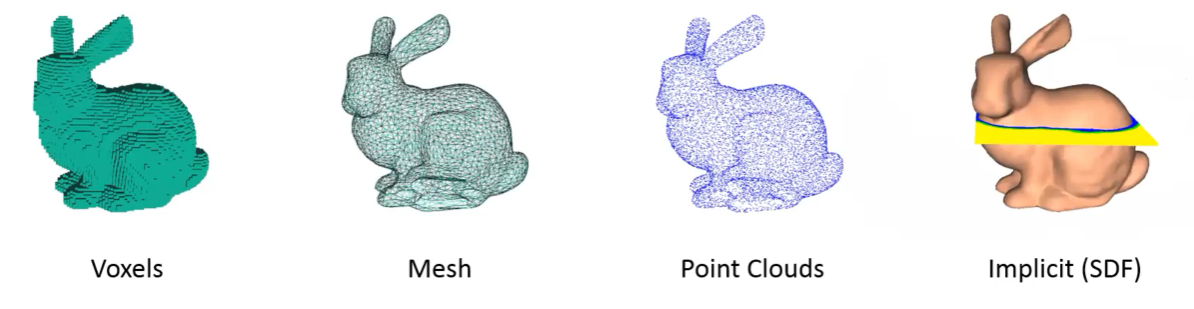
\includegraphics[width=\linewidth]{\imgfp/representations}
%	\caption{Different 3D representations. Voxels comprise uniform axis-aligned grid with occupancy information. Meshes define 3D points and their connectivity into 3D plane patches (polygons). Point clouds define just 3D points. Signed Distance Function for each point in 3D space associates a distance to a surface, points with distance 0 implicitly model a surface. The picture is adapted from \href{https://www.youtube.com/watch?v=r9lvAyAgR3E}{www.youtube.com/watch?v=r9lvAyAgR3E}}
%	\label{lit:fig:3d-representations}
%\end{figure}

\begin{figure}[h!]
	%\fboxrule=2pt
	\centering
	\begin{subfigure}[b]{0.49\textwidth}
		\centering
		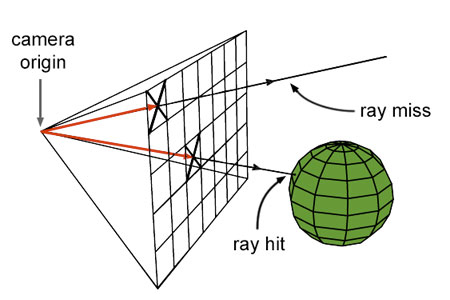
\includegraphics[height=5cm]{\imgfp/raytracing}
		\caption{}
		\label{lit:fig:raytracing}
	\end{subfigure}
	\hfill
	\begin{subfigure}[b]{0.49\textwidth}
		\centering
		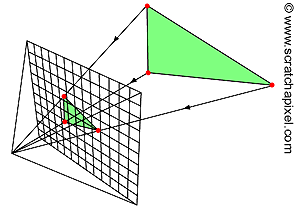
\includegraphics[height=5cm]{\imgfp/rasterization-s}
		\caption{}
		\label{lit:fig:rasterization}
	\end{subfigure}
	
	\caption{(\protect\subref{lit:fig:raytracing}) Rays are cast from the camera origin through each pixel, and if a ray hits any surface, the pixel is colored accordingly. (\protect\subref{lit:fig:rasterization}) In rasterization, vertices of a polygon are projected onto a raster grid, filling the pixels that belong to the projected shape. Images from \href{https://www.scratchapixel.com/}{www.scratchapixel.com}.}
	\label{lit:fig:rendering-methods}
\end{figure}

\section{Neural Rendering and human avatars}\label{lit:nrender}

As was mentioned in the Section \ref{intro:nrender}, any theory that lies inside algorithmic approaches may miss complex correlations in the real world behavior. This can be a corner stone that differentiates realistically-looking and truly photo-realistic images. For this reason, statistical methods of AI (such as DNNs) are applied, to learn a parameterized model from the real observations. In our case, it learns on real photos to synthesize images automatically from descriptive data, such as position of the view in the world, or the desired content in the view. The learning per se comes down to iterative processing of the DNN from input to output, computing loss (fitness) between the output and desired data. The DNN's weights are updated (optimized) using a gradient value of the loss with respect to every weight.

There are two major modes of DNNs training. The first it to learn on diverse data to understand different modalities of it. With this knowledge, a feed-forward with novel inputs would yield an acceptable result \cite{dnn:gan14, dnn:gaugan19, dnn:stylegan-v1-19}. Although time of inference is much smaller than of training, it's still rarely real-time, because such generalization requires a substantial number of learnable parameters. Another approach is optimization-based. A DNN is trained only on a narrow domain of the data, requiring fewer parameters to fit. Every novel domain needs training of a separate model. 

Next, we'll review relevant advances of DNN research for image synthesis. \textit{Multi-Layer Perceptron} (MLP) is a fully-connected neural network, where layers compute weighted sums of a previous layer, and transform sums by a non-linear function \cite{aux:activation18}. MLP is known to be a universal function approximator \cite{dnn:mlp89}, yet high accuracy requires lots of parameters. Still, the research community has found it powerful to use MLPs as an implicit 3D scene representation, and then synthesizing the images using deterministic algorithms, such as ray casting \cite{dnn:scene-repr19}. This idea evolved into \textit{neural radience fields} (NeRF, \cite{dnn:nerf20}), where MLP maps any scene point $(x, y, z)$ and view angle $(\theta, \phi)$ to its color $(r, g, b)$ and volume density $\sigma$. The method can model complex materials and reflections from novel views of static scenes, but takes seconds to query the volume and render an image. It's also suitable for reconstruction of dynamic objects, such as humans\cite{dnn:phorhum22}.

Large MLPs are prone to overfitting, i.e. that they can memorize perfect solutions to the training data and fail to generalize the novel data. \textit{Convolutional Neural Networks} (CNN) revolutionized \cite{aux:cnn98, dnn:alexnet12} image processing with fewer parameters and better generalization. There, a series of 2D convolution operations is applied, that compute weighted sums over input tensors with a small-sized learnable matrix in a sliding-window manner. In MLPs the same data in different places on an image is processed with different weights. CNNs are invariant to spatial shifts, but may have small receptive field - i.e. size of recognized patterns limited by kernel size. Many notable DNNs apply convolutional layers, e.g. AlexNet\cite{dnn:alexnet12} ResNet\cite{dnn:resnet16}, VGG\cite{dnn:vgg14}, U-Net\cite{dnn:unet15}.

\textit{Generative Adversarial Networks} (GAN,  \cite{dnn:gan14}) is an optimization framework for DNNs that advanced image synthesis a lot since CNNs. In essence, it represents a competing game. A generator network $G$ learns the data distribution. A discriminator network $D$ learns to classify input as either real observation, or produced by $G$ (fake). Importantly, the losses for $G$ don't need to measure similarity of the real and generated data, it's enough for $G$ to minimize accuracy of $D$, by making more realistic fakes. Ever since, many GAN models were proposed \cite{survey:gans:18}, the most notable of which is StyleGAN \cite{dnn:stylegan-v1-19,dnn:stylegan-v2-20,dnn:stylegan-v3-21} that is able to generate artificial high-resolution images of human faces, but far from real-time inference and rich articulation. Apart from that, GANs can be a part of architecture to generate any data at training time and optimize with respect to it \cite{dnn:stylepeople21, dnn:hyperstyle21}.

Speaking of DNN optimization, it's desirable to prevent overfitting and at the same time speed up convergence of results to the optimum (escaping underfitting). Overfitting can be prevented with more diverse real data, or by making the existing data diverse via augmenting, e.g. replicating data with varying color, erased content, affine transformations. Also, regularization of weights can be applied to make training harder, e.g. dropout\cite{aux:dropout14} -- random nullifying of activation values; or weight decay\cite{aux:adamw17} -- small decrease of weights towards 0 absolute value on every optimization step.

The reason of underfitting can be a deficit of number of parameters to fit the data. Also, a covariate shift can be frequently observed, e.g. training and novel (test) data may have slightly different distributions, or even activations of internal layers may have different distributions after updating weights of a network. To compensate the shift, normalization techniques are applied. Batch Normalization (BN, \cite{dnn:bn15}) algorithm during training normalizes intermediate activations to the mean and variance of the whole batch of data, see Formula \ref{lit:eq:bn}. Here $\gamma$ and $\beta$ are learned vectors of same size as number of input channels. Besides, the batch statistics are accumulated on each step with exponential averaging, so that during inference batches of any size could be processed. Instance Normalization (IN, \cite{dnn:in16}) follows the same formula, but the statistics are computed over each sample, rather than a batch of samples. These and other normalization schemes may increase DNNs convergence speed and reduce sensitivity to hyperparameters.
\begin{equation}
	\setlength\abovedisplayskip{2pt}y = \frac{x - \mathrm{E}[x]}{\sqrt{\mathrm{Var}[x] + \epsilon}} * \gamma + \beta
	\setlength\belowdisplayskip{2pt}
	\label{lit:eq:bn}
\end{equation}

There is a branch of research called \textit{deferred neural rendering}, where 3D meshes of objects are rendered with a neural texture -- a tensor, that unlike usual textures with 3 color channels (RGB), has generally $C$ channels \cite{dnn:deferred19}. A DNN is trained to map this neural image to a colorful RGB image with segmentation (RGBS/RGBA), see Figure \ref{lit:fig:stylepeople}. The motivation is to give a clue to the DNN on what to synthesize, and to optimize the neural texture to implicitly model specular properties of real materials. Also a coarse mesh of the object can be used, that doesn't model small details, and the DNN will have to put information into the neural texture about reconstruction of these details \cite{dnn:stylepeople21, dnn:anr21}. Crucially, the algorithm that renders the mesh with the neural texture has to be differentiable \cite{survey:diff-render20}, to optimize the texture.

This thesis focuses on human avatars neural rendering, i.e. recovering of photo-realistic appearance, and modeling movements of limbs, face, hair, clothes. The reconstruction may cover the full-body (FB)  \cite{dnn:fb-cloth-avatar21, dnn:stylepeople21, dnn:anr21}, upper-body (UB) \cite{dnn:upper-avatar21}, or only face of a person \cite{dnn:volumetric-primitives21, dnn:hyperstyle21}. The source data may vary, e.g. a single frontal photo (one-shot avatar), multiple photos from sides (few-shot avatar), a video sequence (video-based avatar). Either can be captured on a monocular camera\cite{dnn:stylepeople21}, stereo camera\cite{dnn:stereo-avatars11}, multiple cameras\cite{dnn:volumetric-primitives21, dnn:textured-avatars19}; with or without camera calibration parameters (intrinsics as in Formula \ref{lit:eq:intrinsic}). Images alone impose depth ambiguity, i.e. the true size of objects on an image is unknown. Depending on proximity to the camera, they appear smaller or bigger. It can be resolved with depth sensor information \cite{dnn:depth-avatar11}, or by scanning 3D meshes of objects \cite{dnn:phorhum22}, both requiring expensive equipment. Thus, it's desired to make realistic avatars from common data in-the-wild -- a few images or videos taken on a monocular uncalibrated camera. The task is ill-posed and combining quality with real-time inference is challenging. That said, photo-realism isn't achieved yet. 

We follow StylePeople \cite{dnn:stylepeople21} architecture as a baseline for this thesis. It's based on deferred neural rendering, as described above (see Figure \ref{lit:fig:stylepeople}). The input of a neural renderer network is a rasterized image of a generic human body mesh, that doesn't contain any personal details, such as facial features, hair, clothes. It's rasterized with a neural texture tensor, that has usually between 4 and 16 channels. Feeding this "neural" image through the renderer, the personal features are filled in, and colorful image is returned, along with body contour segmentation. Both neural renderer and neural texture are jointly optimized using image-based losses (more details in Section \ref{lit:metrics}), including an adversarial loss using a discriminator network (see the paragraph on GANs above). 

The neural renderer's architecture is a CNN called U-Net \cite{dnn:unet15}, consisting of an encoder and decoder part. In encoder, input is gradually down-scaled and processed with convolutional filters. In the decoder part the input data and corresponding encoder layer's output are further processed and gradually up-scaled to the original resolution. The resulting output is fed through color and segmentation "heads" to make the final RGBA image. Commonly to improve training, the encoder part is replaced with a powerful CNN backbone, in our case ResNet\cite{dnn:resnet-unet20,dnn:resnet16}. The discriminator's architecture is exactly as in StyleGANv2 \cite{dnn:stylegan-v2-20}, the details of which are irrelevant for this work.

The generic human body model used in StylePeople is \textit{Skinned Multi-Person Linear Model - Expressive} (SMPL-X \cite{dnn:smplx19}, derived from \cite{dnn:smpl15, dnn:smplify16}). It allows representing a variety of human bodies, including expressive faces and hands as 3D triangular meshes with $N = 10475$ vertices, and $K = 54$ joints for limbs, face and fingers (See Figure \ref{lit:fig:smplx}). It does so by learning bodies distribution from many 3D scans of people. A particular body shape is derived as a linear combination of learned body blend shapes $\mathcal{S}=[S_1, ..., S_{\lvert \beta \rvert}] \in \mathbb{R}^{3 N \times \lvert \beta \rvert}$, where $\beta$ is a vector of linear coefficients. The body blend shapes are orthonormal principle components of the learned mesh vertex displacements. Typically, about 10 body shape components are enough for reconstruction of any body constitution. Face vertices have their own blend shapes $\mathcal{E}=[\mathcal{E}_1, ..., \mathcal{E}_{\lvert \psi \rvert}]$, combined with $\psi$ coefficients, similarly about 10 are usually enough.

Body mesh can be posed using learned orthonormal components $\mathcal{P}=[P_1, ..., P_{9K}] \in \mathbb{R}^{3 N \times 9 K}$ of vertex displacement with respect to a pose. The pose is defined by axis aligned rotations of body joints $\theta$ ($\lvert \theta \rvert = 3 K$). It's then expanded into rotation matrices $K \times 3 \times 3$ using Rodrigues formula \cite{aux:rodrigues11}, notated further as $R : \mathbb{R}^{\lvert \theta \rvert} \rightarrow \mathbb{R}^{9 K}$. The computed body shape offsets, face shape offsets and pose offsets are simply added to an average body mesh $\bar{T}$ in a default pose $\theta^{*}$. Formally, a posed triangular mesh $T_p$ can be obtained as:

\setlength\abovedisplayskip{0pt}
\noindent
\begin{equation}
	\setlength\abovedisplayskip{0pt} T_p(\beta, \theta, \psi) = \bar{T} + B_S(\beta; \mathcal{S}) + B_E(\psi; \mathcal{E}) + B_P(\theta; \mathcal{P})
\end{equation}
\begin{equation}
	B_S(\beta; \mathcal{S}) = \sum_{n=1}^{\lvert \beta \rvert}\beta_n S_n, 
	\quad
	B_E(\psi; \mathcal{E}) = \sum_{n=1}^{\lvert \psi \rvert}\psi_n \mathcal{E}_n
	\quad
	B_P(\theta; \mathcal{P}) = \sum_{n=1}^{9K} \left( R(\theta)_n - R(\theta^{*})_n \right) P_n
\end{equation}
\setlength\belowdisplayskip{0pt} 

SMPL-X also solves issues of mesh deformations and self-intersections, e.g. in poses with bent arms or rotated neck. However, it's computationally expensive to compute and may be skipped, since the neural rendering may handle these artifacts. SMPL-X also proposes an algorithm for optimization-based fitting of the body model to a single image, which is used in StylePeople too. 

\begin{figure}[h!]
	%\fboxrule=2pt
	\centering
	\begin{subfigure}[b]{0.39\textwidth}
		\centering
		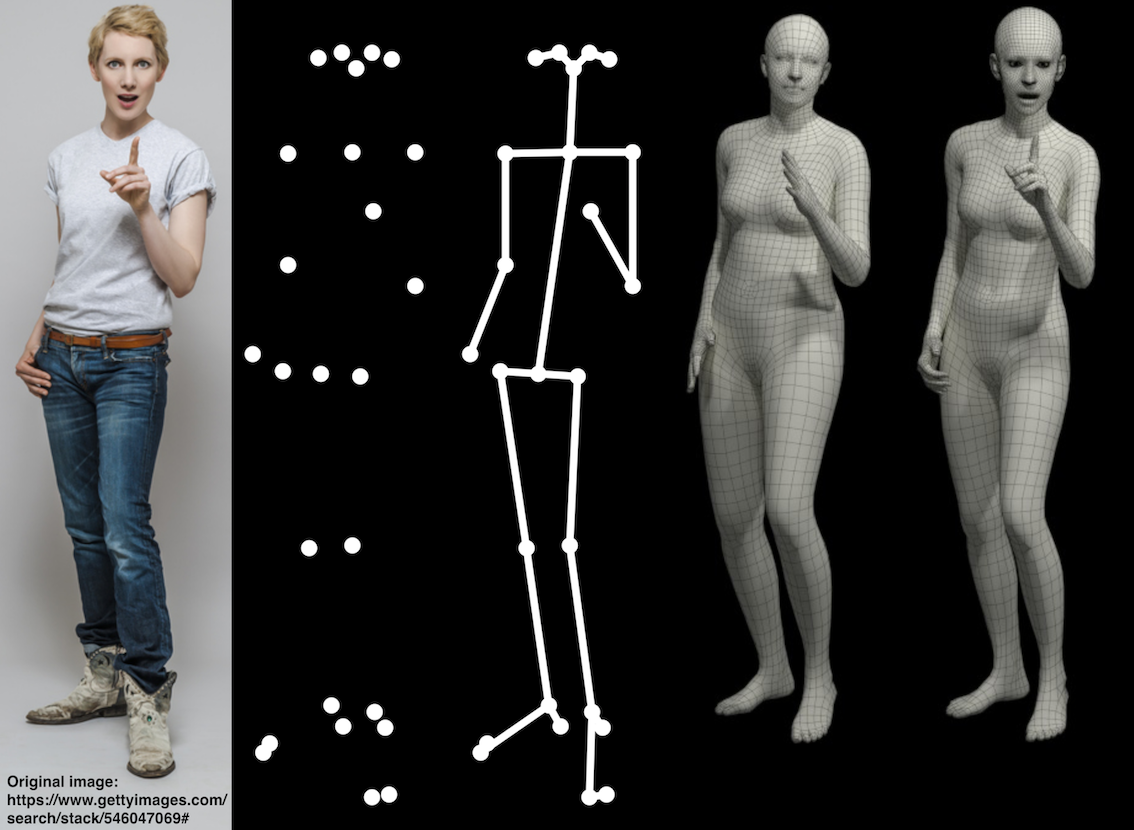
\includegraphics[width=\textwidth]{\imgfp/smplx}
		\caption{}
		\label{lit:fig:smplx}
	\end{subfigure}
	\hfill
	\begin{subfigure}[b]{0.60\textwidth}
		\centering
		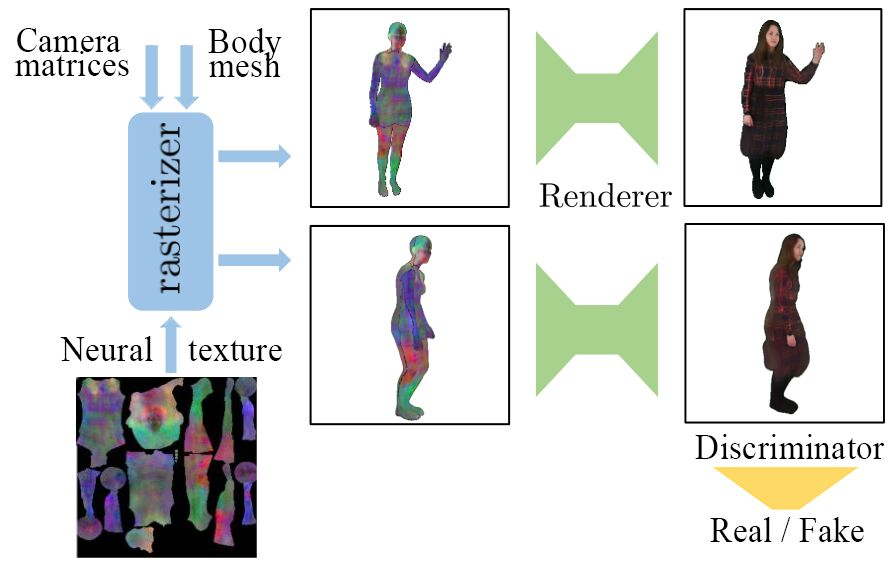
\includegraphics[width=\textwidth]{\imgfp/stylep}
		\caption{}
		\label{lit:fig:stylepeople}
	\end{subfigure}
	\label{lit:fig:avatars}
	\caption{(\protect\subref{lit:fig:smplx}) SMPL-X body model results. Joints are predicted in image space, then body shape and 3D pose are fit to maximize alignment with the source image. The final mesh is generic, lacking person-specific features as hair and clothes. (\protect\subref{lit:fig:stylepeople}) StylePeople data flow. SMPL-X body mesh is rasterized with the neural texture, the image is then refined by a neural renderer, to fill in the person's appearance, clothes, hair. A discriminator network adds supervision to the renderer, by classifying generated and real images of the person. Images adapted from \cite{dnn:smplx19} and \cite{dnn:stylepeople21}.}
\end{figure}

\section{Metrics of image similarity}
\label{lit:metrics}

For comparison of real and synthesized images, many metrics can be applied. Those that are differentiable and fast to compute, are usually used as training losses, by minimizing which the DNN learns how to generate images similar to the real. The next description will follow the notation: $\bmr{f}$ - a fake synthesized image, $\bmr{r}$ - a real image, $\bmr{f}_{segm}$/$\bmr{r}_{segm}$ - their segmentation masks, $\bmr{A_f}$/$\bmr{A_r}$ - intermediate DNN layers activations when processing fake and real images respectively.

\textit{Mean Absolute Error} (MAE or L1 \cite{metric:l1-95}, ideal value 0) measures absolute differences between corresponding pixels. It simplifies the training process, by pushing pixels to equality, but doesn't capture many image degradation effects like blur, warping, etc: 
\begin{equation}
	\setlength\abovedisplayskip{2pt}\text{MAE}(\bmr{f}, \bmr{r}) = \frac{1}{N}\sum_{i=1}^{N}\lvert \bmr{f}_i - \bmr{r}_i \rvert \in [0, +\infty]\setlength\belowdisplayskip{2pt}
\end{equation}

\textit{Mean Squared Error} (MSE or L2 \cite{metric:l1-95}, ideal value 0) measures squared differences between corresponding pixels. In terms of image comparison, similar to MAE. However, it has smoother values distribution, and penalizes high differences much more, which is sometimes harmful. For example, a single pixel may be very different, but it's hardly seen by a human, thus should not be necessarily penalized. 
\begin{equation}
	\setlength\abovedisplayskip{2pt}\text{MSE}(\bmr{f}, \bmr{r}) = \frac{1}{N}\sum_{i=1}^{N}(\bmr{f}_i - \bmr{r}_i)^2 \in [0, +\infty]\setlength\belowdisplayskip{2pt}
\end{equation}

\textit{Learned Perceptual Image Patch Similarity} (LPIPS \cite{metric:lpips18}, ideal value 0) is based on an observation, that image-based neural networks (commonly VGG \cite{dnn:vgg14}) tend to learn inside their weights structured patterns from images. Given a new image, activations of the network will contain a proportion of those patterns that can be found on the image. Thus, we could infer such network with fake and real images, and compare activations. If they're identical, then the original images are perceptually similar on a global level. The difference in activations is applied as a loss during training. The metric is computed as an average MSE distance between corresponding activations (also normalized by the tensors size to equalize contribution of deep layers).
\begin{equation}
	\setlength\abovedisplayskip{0pt} 
	\text{LPIPS}(\bmr{f}, \bmr{r}) = \frac{1}{L}\sum_{l=1}^L \frac{1}{\text{size}(\bmr{A_f}^l)}\text{MSE}(\bmr{A_f}^l, \bmr{A_r}^l) \in [0, +\infty], L \text{ is number of VGG layers} \setlength\belowdisplayskip{0pt}
\end{equation}
	
\textit{Structural Similarity} (SSIM \cite{metric:ssim04}, ideal value 1) metric is based on an idea, that perception of noise on an image is dependent on luminance (mean of image values $\mu$), contrast (standard deviation of image values $\sigma$) and structure (covariance between images $\sigma_{xy}$). The metric is computed for two images from components, that measure luminance difference ($l(\bmr{f}, \bmr{r})$), contrast difference ($c(\bmr{f}, \bmr{r})$), structure difference ($s(\bmr{f}, \bmr{r})$)). Importance of components is also controlled by $\alpha$, $\beta$, $\gamma$ powers.
\begin{equation}
	\setlength\abovedisplayskip{6pt} 
	\begin{aligned}
	& l(\bmr{f}, \bmr{r}) = \frac{2 \mu_{\bmr{f}} \mu_{\bmr{r}} + C_1}{{\mu_{\bmr{f}}}^2 + {\mu_{\bmr{r}}}^2 + C_1} \quad
	c(\bmr{f}, \bmr{r}) = \frac{2 \sigma_{\bmr{f}} \sigma_{\bmr{r}}+ C_2}{{\sigma_{\bmr{f}}}^2 + {\sigma_{\bmr{r}}}^2 + C_2} \quad
	s(\bmr{f}, \bmr{r}) = \frac{\sigma_{\bmr{f}\bmr{r}} + C_2/2}{\sigma_{\bmr{f}}\sigma_{\bmr{r}} + C_2/2} \\
	& \text{SSIM}(\bmr{f}, \bmr{r}) = 
	[l(\bmr{f}, \bmr{r})]^\alpha \cdot
	[c(\bmr{f}, \bmr{r})]^\beta \cdot
	[s(\bmr{f}, \bmr{r})]^\gamma \in [-1;1]
	\end{aligned}
	\setlength\belowdisplayskip{6pt}
\end{equation}
where $C_1 = (K_1L)^2$, $C_2 = (K_2L)^2$,  $L$ is a range of values stored in pixel channels (usually it's 1 for channels in floating-point format, or 255 for integer 8-bit channel format), $K_1$ and $K_2$ are arbitrary constants to ensure numerical stability for near-zero denominator. SSIM is usually computed in a $11 \times 11$ sliding window and averaged over the whole image. It can detect degradation due to noise, but might be insensitive to blur and color shift.

\textit{Multi-Scale Structural Similarity} (MS-SSIM \cite{metric:msssim03}, ideal value 1) is an extension of SSIM, but contrast and structure terms are computed on multiple scales, i.e. the original images are processed with a low-pass filter and downsampled by a factor of 2, a total of $M$ times. All the computed multi-scale components are multiplied to the metric. The metric was shown to be the same or better than SSIM in detecting many types of distortions:
\begin{equation}
	\setlength\abovedisplayskip{0pt} 
	\text{MS-SSIM}(\bmr{f}, \bmr{r}) = 
	[l(\bmr{f}, \bmr{r})]^\alpha \cdot
	\prod_{j=1}^{M}
	[c_j(\bmr{f}, \bmr{r})]^{\beta_{j}}
	[s_j(\bmr{f}, \bmr{r})]^{\gamma_j} \in [-1;1] \setlength\belowdisplayskip{0pt} 
\end{equation}

	
\textit{Peak Signal-to-Noise ratio} (PSNR \cite{metric:psnr13}, ideal value $+\infty$) metric comes from signal processing theory. It captures a ratio of the maximum value in an noise-free signal to the average noise magnitude (can be captured by MSE). The metric indeed helps to detect noise levels, but it's much less useful as image similarity measure than other metrics, such as SSIM.
\begin{equation}
	\setlength\abovedisplayskip{0pt} 
	\text{PSNR}(\bmr{f}, \bmr{r}) = 20 \cdot \log_{10} \left( \max(\bmr{r}) \right) - 10 \cdot \log_{10}\left( \text{MSE}(\bmr{f}, \bmr{r}) \right) \in \mathbb{R} \setlength\belowdisplayskip{0pt} 
\end{equation}
	
\textit{Adversarial} loss (GAN-loss \cite{dnn:gan14}, ideal value 0.5) is used as a part of Generator - Discriminator DNN training architecture. It measures how well the discriminator learned to distinguish real images from fake (by assigning probabilities of realism: 0 is fake, 1 is real). The generator's task is to synthesize images that cannot be detected by the discriminator. Ideally, discriminator should report probability 0.5 on average, indicating that it essentially reports a random guess.

\textit{Feature matching} loss (ideal value 0, \cite{metric:fm16}) is analogous to LPIPS, but the intermediate activations on fake and real images are taken not from external image network, but from discriminator network. The motivation is that the generator network will learn to produce images that are perceived as real by the discriminator.

\textit{Dice} loss (ideal value 1, \cite{metric:dice17}) is widely used in various pixel segmentation tasks to learn segmentation masks. It maximizes area of masks intersection and minimizes union of the areas (to prevent false positives in the predicted mask). The formula treats masks as sets of pixels where segmentation value is greater than 0.
\begin{equation}
	\setlength\abovedisplayskip{0pt} 
	\text{Dice}(\bmr{f}_{segm}, \bmr{r}_{segm}) = \frac{2 \lvert \bmr{f}_{segm} \cap \bmr{r}_{segm} \rvert}{ \lvert \bmr{f}_{segm} \rvert + \lvert \bmr{r}_{segm} \rvert} \setlength\belowdisplayskip{0pt} 
\end{equation}

\section{Ways of speeding up DNN inference}
\label{lit:dnn-speedup}

State-of-the-art DNN methods indeed achieve high quality results, but may also have tremendous computational costs. As an example, the models of natural language processing may surpass billions of trained parameters (weights): Turing-NLG has 17 billion parameters \cite{dnn:turingnlg20}, GPT-3 - 175 billion \cite{dnn:gpt3-20}, Megatron-Turing NGL - 530 billion \cite{dnn:megatron22}. This number affects the amount of required computer memory, as all the parameters, computed values (activations) of intermediate DNN layers, and analytic gradients need to be stored. Secondly, sufficient computing power is needed to make training time more feasible. For instance, a computing cluster of 10000 GPUs, 285000 CPU cores was built in order to train GPT-3, still requiring more than a month of constant training \cite{aux:openai-cluster-20}. 

After training, the amount of minimum computing power to perform DNN inference is generally a lot smaller, because we can load and compute neural layers one by one without storing intermediate activations. Nevertheless, inference may still require dozens of GPUs, a handful of memory and seconds to compute. Thus, a few research directions of Deep Learning are dedicated to reduce the required computing power, trying to preserve the similar model's quality.

One such approach is known as \textit{knowledge distillation}. Its idea, is that the learned values of DNN's parameters are not equivalent to knowledge of how to perform a task. In fact, by knowledge we can consider any sufficiently good mapping from input data to the desired output data \cite{method:distillation15}. Thus, we could try to train the original model fully to yield great results, and then to train another DNN "student" model with much fewer parameters. Both models are inferred with the same input data, and the student model is supervised to output the same results as the original model. Mimicking intermediate activations of the original model is also an option to replicate even more knowledge. The simplified neural architecture of the student models helps to reduce computation time and overfitting. That's because with fewer parameters there's less capacity in the student to remember the training data, and also imperfections of the original model's predictions additionally regularize the student \cite{survey:distillation21, speed:distillgan19}. However, knowledge distillation adds up more research work, with experimentation on neural architectures of the student, the training routines and hyper-parameters.

There's an adjacent group of methods, called \textit{neural architecture search}. It aims to automatically find a DNN architecture that would outperform hand-crafted architectures on the given tasks. The motivation is to both reduce the committal effect of selecting a sub-optimal neural architecture by researchers, and to also reduce the amount of parameters required to accomplish the same tasks \cite{survey:neural-arch-search19, dnn:eff-neural-arch-search18}. However, a single search step requires to train the current network, collect quality metrics and then update the architecture. The convergence may require dozens of steps. This limits neural architecture search to lightweight DNNs, and it's hard to apply for big neural architectures.

Another option comes from an observation, that some activation values of DNNs may be less important to the overall output than the others. Such activation values usually have low variance with respect to different input data, i.e. they frequently yield similar values. The corresponding learned parameters could then be replaced in the architecture by constants, if the quality doesn't decrease much. Such approach is called \textit{pruning}. Similarly to knowledge distillation, it allows to train a big model with the full capacity, which eases training. Then the obtained knowledge is squeezed to the lower number of parameters  \cite{method:pruning16, survey:pruning20, speed:prunning-gan21}.

On a computer hardware level, DNNs are usually trained and inferred with weights and activations represented with 16-bit/32-bit floating point numbers (also referred to as half-float or FP16; full-float or FP32 respectively). A \textit{quantization} approach switches to integer number formats, with lower memory usage, e.g. 4-bit/8-bit/16-bit integer numbers (INT4/INT8/INT16). The main motivation is that integer operations can be computed faster than floating-point ones, their physical circuits are smaller, thus decreasing device's size, overheating, energy consumption \cite{aux:fp-int-speed10}. The quantization approach relies on a fact, that a vector of floating-point numbers $\bm{x}$ can be approximately expressed as 
\begin{equation}
	\setlength\abovedisplayskip{0pt}
	\bm{x} \approx s^\prime_{\bm{x}} \cdot \bm{x^\prime_{\mathtt{int}}} = s_{\bm{x}} \cdot (\bm{x_{\mathtt{int}}} - z_{\bm{x}})
	\setlength\belowdisplayskip{0pt}
\end{equation} where $s^\prime_{\bm{x}}$ is a floating-point scalar, $\bm{x^\prime_{\mathtt{int}}}$ contains only integer values. Then they can be reformulated using an integer zero-offset $z_{\bm{x}}$, so that values in $\bm{x_{\mathtt{int}}}$ are mapped uniformly to range $(0, 2^b-1)$, with $b$ being bit-width of a number. Having a floating-point vector $\bm{x}$, it's quantized as:  
\begin{equation}
	\setlength\abovedisplayskip{0pt}
	\bm{x_{\mathtt{int}}} = \text{round}(\bm{x}/s_{\bm{x}}) + z_{\bm{x}}
	\setlength\belowdisplayskip{0pt}
\end{equation}

Since many operations in neural networks can be computed using dot products of vectors, this allows to represent them in a quantized form. For example, a basic operation of matrix-vector multiplication with a floating-point weights matrix $\bm{W}_{n \times m}$ and a bias vector $\bm{b}_n$. The output activation vector $\bm{A}_n$  could be computed from an input activation vector $\bm{x}_m$ as:
\setlength\abovedisplayskip{0pt}
\begin{align}
\begin{split}
	\bm{A} &= \bm{b} + \bm{W} \bm{x}\\
  &\approx \bm{b}
  + [s_{\bm{w}} (\bm{W}_{\mathtt{int}} - z_{\bm{w}})]
  \cdot [s_{\bm{x}} (\bm{x}_{\mathtt{int}} - z_{\bm{x}})] \\
  &=\bm{b}
  + s_{\bm{w}} s_{\bm{x}} ( 
  \bm{W}_{\mathtt{int}} \bm{x}_{\mathtt{int}}
  - \bm{x}_{\mathtt{int}} z_{\bm{w}}
  \textcolor{blue}{- \bm{W}_{\mathtt{int}} z_{\bm{x}}
  + z_{\bm{x}} z_{\bm{w}}}).
	\setlength\belowdisplayskip{2pt}
\end{split}
\end{align} The last two terms shown in blue can be pre-computed for the whole DNN, and merged with the bias vector $\bm{b}$ \cite{dnn:quant-white21}. However, since there's still an extra overhead from computation of $\bm{x}_{\mathtt{int}} z_{\bm{w}}$, specifically for weights it's common to use symmetric quantization, where floating-point values are mapped to $(-2^{b-1}, 2^{b-1}-1)$ integer range, with floating-point 0 mapped precisely to integer 0, thus making $z_{\bm{w}} = 0$, and eliminating the overhead. 

Typically, a post training quantization (PTQ) is applied to weights and activations of a DNN, because a complete experiment can be quantized via a provided software tool, and automatically be sped up from quantized computations. On the other hand, if precision of the outputs is a priority, a  quantization-aware training (QAT) \cite{quant:qat18} approach is used. Here architecture tweaks are required to do quantized inference and weights updates, with an idea to make the model learn to deal with the quantization imprecision. As a downside, it enlarges training time and adds issues with analytic gradients back-propagation through rounded values \cite{quant:straight-through-estimator13}.

Usually, the uniform quantization is appealing for simplicity of hardware implementation. However, the quantization range defined by constants $s$ and $z$ may be selected too wide, e.g. min-max range of values in a tensor with existing outliers. Thus, a lot of precision will be lost as different numbers will be mapped to the same integer value. Instead, the range can be selected to minimize MSE with respect to the original floating-point values \cite{quant:mse19, speed:quant-error-analysis15}. If hardware supports it, instead of defining per-tensor quantization constants, they can be defined per-channel for more precision. Alternatively, a Cross Layer Equalization \cite{quant:cle20} can be applied to re-parameterize quantized weights and biases, compensating the channels' discrepancy of ranges, without adding runtime overhead. A non-uniform quantization can also be used to devote more precision to near mean values, and less to the outliers, but the hardware support of it is very limited \cite{quant:non-uniform21}.

Moving on, DNNs also suffer from computational inefficiency, when similar input data leads to computing identical activations of layers. The DNN's architecture can be designed to cache and reuse these values. It can be applied to video stream processing or synthesis, where multiple consecutive frames have similarity \cite{aux:reusing19}. Additionally, filters of CNNs may frequently contain repeated weights after being quantized. Thus, as a filter slides over the data, certain dot-products can be reused \cite{dnn:reusing18}. While having a potential to speed up a certain DNN architecture, it requires immense manual hand-craft, which slows down active research and experimentation.

The last but not least appoach, is to design the neural architectures efficiently, i.e with a good trade off of inference speed and outputs accuracy. It's obtained by reducing the number of parameters, applying only fast-to-compute neural layers, and composing them into a sparse computational graph. It leads to a better utilization of memory caches and computing cores of the hardware. Often, such models are implemented using low-level parallelized code, that increases the number of floating-point operations per second (FLOPs) even further. The notable examples are: MobileNetV1 \cite{dnn:mnv1-17}, MobileNetV2 \cite{dnn:mnv2-18}, MobileNetV3 \cite{dnn:mnv3-19},  ShuffleNetV1 \cite{dnn:shufflenetv1-18}, ShuffleNetV2 \cite{dnn:shufflenetv2-18}, CondenseNetV1 \cite{dnn:condensenetv1-18}, CondenseNetV2 \cite{dnn:condensenetv2-21}, EfficientNet \cite{dnn:efficientnetv1-19}. Although the original papers obtain similar or better results with their proposed architectures, the drop-in replacement is not guaranteed for every task. In this work a significant drop of quality is observed, when a baseline ResNet18 backbone was replaced with either MobileNetV2 or EfficientNet.

%

\section{Computations on mobile hardware}
\label{lit:mobile}

Traditional desktop computers have hardware, where components are designed to be independent and replaceable. This is achieved through standardization of connectors and signaling. This design is convenient when physical size of devices, power usage, or necessity of active cooling are not issues. On the other hand there is mobile hardware, which can be found in modern smartphones, watches, AR and VR devices. There exists a strong desire to minimize physical size, weight, battery power usage and heat generation. Despite the wide variety of mobile devices and vendors, the state-of-the-art mobile architectures look similar on a high level. They are presented as Systems-on-a-chip (SoC), also referred to as heterogeneous platforms, where computing devices of different underlying principles are fused under a single silicon. The computing work is offloaded to the designated computing devices, to minimize idleness and latency. Such platforms may accelerate general computing (CPU), graphics computing (GPU), signal processing, networking, cryptography, external devices, camera processing, AI computing, sensing, etc. To name a few SoC platforms, there are: Nvidia Tegra \cite{soc:nvidia-tegra}, Samsung Exynos \cite{soc:exynos}, Qualcomm Snapdragon \cite{soc:snapdragon}. Notably, all of them advance towards providing special computing devices for AI, and DNNs in particular \cite{mobile:dl-review19}. Such AI accelerators can come by the names: Deep Learning Accelerator, Neural Processing Unit (NPU), Tensor Processing Unit (TPU), etc \cite{soc:tops}. This work by default targets devices running Qualcomm Snapdragon SoC.

The latest chip called Qualcomm Snapdragon 888 consists of an 8-core CPU, a GPU with mixed precision AI inference support (vectorized half-float/full-float), a sensing processor, and a Digital Signal Processor (DSP). The latter is especially optimized for parallel integer computations, which are common in real-time 1D or 2D digital signal processing (e.g. Fast Fourier Transform algorithm). It supports parallel scalar, vector and tensor operations, while retaining state-of-the-art low level of power usage. Besides, it's possible to use DSP as an AI accelerator to infer a quantized DNN, and get massive benefit in inference speed and energy consumption. All accelerators of the SoC are located on the same chip and have access to shared memory, allowing to reduce overhead of data transfer (which is common in desktop systems). The claimed performance of the combined accelerators is 26 TOPS (Trillion Operations per Second). The platform also offers a triple-core chip for multithreaded camera processing with up to 2.7 Gigapixels per second of throughput \cite{soc:snapdragon888}.

Importantly for this work, Qualcomm Snapdragon's DSP works with tensors layout called BHWC (Batch-Height-Width-Channel), that is, the data of a single spatial element (pixel) is stored contiguously (e.g. $C$ values for a pixel 1 are followed by $C$ values for a pixel 2, and so on). This will be utilized during real-time input data generation for the DNN researched in this work. The other possible format is BCHW (Batch-Channel-Height-Width), which is usually used in software libraries for DNN training on desktop computers.

As well as usual quantization approaches described in Section \ref{lit:dnn-speedup}, for Snapdragon DSP a data-free quantization algorithm is implemented, which doesn't require estimating quantization ranges from example input dataset \cite{speed:datafreequant19}. It features high quantization speed, which used to be critical with big datasets, and also achieves near-identical outputs' quality for quantized DNNs.

An AI model can possibly provide software level improvements for better hardware utilization. For example, the work \cite{mobile:pipelining20} suggests a pipeline approach, where a model is split into several stages. Instead of processing input from start to finish, each stage receives new input as soon as it finished the previous calculation. By combining usage of multiple accelerating devices on mobile hardware, it's possible to almost double real time performance.

